% Introduzir a base teórica da DTFT, suas propriedades e como a FFT é usada para implementá-la em ambiente discreto e computacional.

A DTFT é uma extensão da transformada de Fourier para sinais discretos, convertendo um sinal no domínio do tempo em uma representação no domínio da frequência. Ela fornece uma descrição das componentes de frequência de um sinal amostrado e é amplamente utilizada em processamento digital de sinais (PDS). No entanto, a DTFT, como uma transformada contínua no domínio da frequência, é impraticável de calcular diretamente em sistemas digitais e, por isso, é frequentemente aproximada pela Transformada Discreta de Fourier (DFT).

A DFT converte um sinal amostrado em um número finito de componentes de frequência, dividindo o sinal em $N$ pontos uniformemente distribuídos no espectro, onde $N$ é o número de amostras do sinal. Essa transformada é definida matematicamente como:

$$
X[k] = \sum_{n=0}^{N-1} x[n] \cdot e^{-j \frac{2 \pi k n}{N}}, \quad k = 0, 1, \dots, N-1
$$

onde $X[k]$ representa as componentes de frequência e $x[n]$ são os valores do sinal amostrado. Essa expressão calcula diretamente cada ponto de frequência, mas é computacionalmente intensiva quando $N$ é grande, pois exige $O(N^2)$ operações.

\subsection{Propriedades da DTFT e DFT}

Algumas propriedades importantes da DTFT e DFT incluem:

\begin{itemize}
    \item \textbf{Periodicidade}: Ambas são periódicas no domínio da frequência. A DTFT é uma função contínua e periódica com período $2\pi$, enquanto a DFT tem periodicidade de $N$ pontos no domínio discreto.
    \item \textbf{Simetria}: Para sinais reais, a DTFT e a DFT produzem espectros simétricos em torno da frequência zero, simplificando a análise ao focar apenas em metade do espectro.
    \item \textbf{Linearidade}: Ambas são transformadas lineares, permitindo a combinação de sinais transformados.
    \item \textbf{Propriedade da Convolução}: A convolução no domínio do tempo corresponde a uma multiplicação no domínio da frequência, útil para analisar sistemas lineares e invariantes no tempo.
\end{itemize}

\subsection{FFT e Implementação Computacional}

A Transformada Rápida de Fourier (FFT) é um algoritmo que calcula a DFT de forma eficiente, reduzindo a complexidade computacional para $O(N \log N)$. A FFT divide a DFT em operações menores, usando recursivamente a simetria e periodicidade dos exponenciais complexos. Essa abordagem é especialmente útil em sinais com número de amostras que são potências de dois, permitindo uma subdivisão rápida e precisa dos cálculos necessários para transformar o sinal.

No ambiente computacional, como no Octave, a FFT é aplicada diretamente a sinais discretos, produzindo uma aproximação da DTFT. A resolução e precisão do espectro dependem do número de amostras e da frequência de amostragem, que devem ser adequadamente escolhidos para garantir uma representação fiel do sinal original sem aliasing.


\subsection{Aplicação da DTFT}
Quando aplicamos uma janela $w[n]$ ao sinal, o sinal janelado é dado por:
$$
   x_w[n] = x[n] \cdot w[n]
$$
onde $w[n]$ é uma função de janela de tamanho $N$, usada para minimizar os efeitos de vazamento espectral. Exemplos comuns de janelas incluem a janela de Hamming, Hann, e retangular.

A DTFT do sinal janelado, $X_w(e^{j \omega})$, é dada pela convolução da DTFT do sinal original $X(e^{j \omega})$ com a DTFT da janela $W(e^{j \omega})$:
$$
   X_w(e^{j \omega}) = X(e^{j \omega}) * W(e^{j \omega})
$$

\subsection*{DTFT do Sinal Sem Janela}

Para referência, a DTFT do sinal original $x[n] = C + A \cos(2 \pi \alpha n)$ (sem janela) pode ser calculada como a soma das DTFTs de cada termo:

1. \textbf{DTFT da componente DC} $C$:
$$
   X_{\text{DC}}(e^{j \omega}) = C \cdot 2 \pi \delta(\omega)
$$

2. \textbf{DTFT da componente cossenoidal} $A \cos(2 \pi \alpha n)$:

Podemos expressar o cosseno em termos de exponenciais complexas:
$$
   A \cos(2 \pi \alpha n) = \frac{A}{2} \left( e^{j 2 \pi \alpha n} + e^{-j 2 \pi \alpha n} \right)
$$
Assim, a DTFT dessa parte é:
$$
   X_{\cos}(e^{j \omega}) = \frac{A}{2} \cdot 2 \pi \left( \delta(\omega - 2 \pi \alpha) + \delta(\omega + 2 \pi \alpha) \right)
$$

3. \textbf{DTFT do sinal total} $x[n]$:
$$
   X(e^{j \omega}) = C \cdot 2 \pi \delta(\omega) + \frac{A}{2} \cdot 2 \pi \left( \delta(\omega - 2 \pi \alpha) + \delta(\omega + 2 \pi \alpha) \right)
$$

\subsection*{DTFT do Sinal Janelado}

Quando a janela $w[n]$ é aplicada, o espectro do sinal janelado $X_w(e^{j \omega})$ é a convolução do espectro do sinal $X(e^{j \omega})$ com o espectro da janela $W(e^{j \omega})$:
$$
   X_w(e^{j \omega}) = X(e^{j \omega}) * W(e^{j \omega})
$$

\subsection*{Computacionalmente}
No Octave, aplicamos a função da FFT para obter uma aproximação da DTFT, como mostra o exemplo abaixo.

\lstinputlisting[language=Octave]{02_analytic_development/example_fft.m}
\begin{figure}[H]
   \centering
   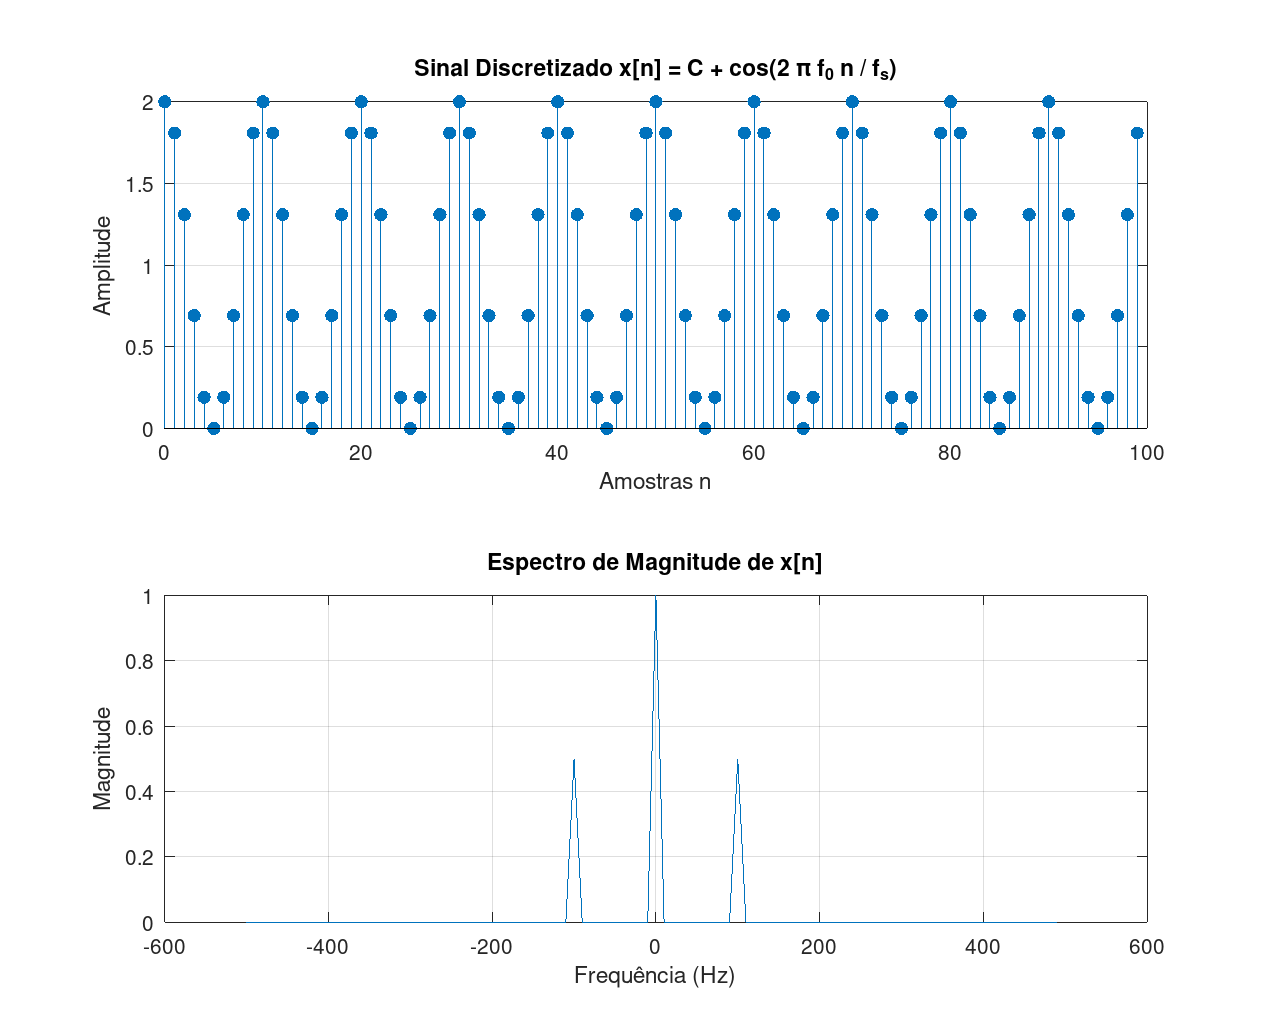
\includegraphics[width=1\linewidth]{02_analytic_development/example_fft.png}
   \caption{Sinal e Espectro de Magnitude}
   \label{fig:enter-label}
\end{figure}


\subsection{Configuração do Experimento}
O processo de geração e captura do sinal foi implementado utilizando o microcontrolador \textbf{Arduino ATmega 2560}, com as seguintes configurações específicas:

\begin{itemize}
    \item \textbf{Geração do Sinal}:
        \begin{itemize}
            \item \textbf{Amplitude de Pico a Pico (Vpp)}: 5V, para se adequar ao limite de entrada do ATmega 2560.
            \item \textbf{Offset de 2.5 V}: Foi aplicado um offset de 2.5V ao sinal, mantendo-o dentro do intervalo de 0 a 5V, que é o intervalo suportado pelo conversor analógico-digital (ADC) do Arduino.
        \end{itemize}
    
    \item \textbf{Configuração da Frequência de Amostragem}:
        \begin{itemize}
            \item A frequência de amostragem ($F_s$) foi configurada em valores variados: \textbf{50 kHz, 20 kHz, 10 kHz, 5 kHz e 2 kHz}.
            \item A configuração da frequência de amostragem foi realizada por meio de ajustes nos \textbf{registradores internos do Arduino}, permitindo o controle direto sobre o tempo de amostragem e a frequência.
        \end{itemize}

    \item \textbf{Envio de Dados pela Porta Serial}:
        \begin{itemize}
            \item Após cada ciclo de amostragem, o Arduino envia os dados obtidos para a porta serial. Esse envio é realizado no seguinte formato:
            \begin{center}
                \texttt{"Fs:totalSamplings;"}
            \end{center}
            onde:
            \begin{itemize}
                \item \textbf{Fs} representa o valor da frequência de amostragem usada.
                \item \textbf{totalSamplings} é o número total de amostras coletadas.
            \end{itemize}
        \end{itemize}
    
    \item \textbf{Processamento do Sinal no Octave}:
        \begin{itemize}
            \item Os dados recebidos na porta serial são capturados no software \textbf{GNU Octave} para processamento. No Octave, os valores de $F_s$ e \textit{totalSamplings} são utilizados para análise espectral do sinal, permitindo visualizar o conteúdo em frequência do sinal capturado e verificar a eficácia da amostragem para cada configuração de $F_s$.
        \end{itemize}
\end{itemize}

Essas configurações permitiram um controle preciso do processo de captura de sinal e garantiram que os dados fossem corretamente armazenados e transmitidos para análise subsequente.


